\documentclass[a4paper, margin=2cm, 11pt]{article}
\usepackage[utf8]{inputenc}
\usepackage{fontspec}
\setmainfont{Arial}
\usepackage{setspace}
\usepackage{lineno}
\usepackage{natbib}
\renewcommand\bibsection{\section{Cited References}}
\setcitestyle{citesep={;}, aysep={,}}
\usepackage{pgfgantt}
\usepackage{xcolor}
\usepackage{ragged2e}
\definecolor{duckegg}{HTML}{CAE8DC}

\title{Thesis Proposal}
\author{Talia Al-Mushadani}
\date{April 2019}

\begin{document}

\begin{onehalfspacing}
\begin{titlepage}
    \begin{center}
        \Huge
        \textbf{Detecting Selection from Longitudinal Deep Sequencing Data in Viruses}
        
        \vspace{2cm}
        \LARGE
        \textbf{Bhavin Khatri}
        \\
        \textsl{bkhatri@imperial.ac.uk}
        \vspace{0.5cm}
        \\
        \textbf{in collaboration with Matteo Fumagalli}
        \\
        \textsl{m.fumagalli@imperial.ac.uk}
        
        \vspace{9cm}
        \LARGE
        \textbf{Talia Al-Mushadani}
        \\
        \textsl{ta1915@ic.ac.uk}
    \end{center}
\end{titlepage}

\linenumbers

\section{Keywords}
\textsl{Evolutionary Virology, Population Genetics, Natural Selection, \\ Machine Learning, Norovirus} 

\section{Introduction to Project \& Proposed Questions}
Currently research into how the Norovirus genome evolves via selection has been limited in scope \citep{Steyer2018} due to the lack of longitudinal deep-sequencing data on the virus and the lack of a simple methods to assess where in the genome selection is occurring. This project will be using longitudinal deep-sequencing data of Norovirus in patients, provided by Prof. Judith Breuer at UCL/GOSH, and will compare two streamlined identification methodologies. The two main methods that will be compared are a heuristic approach \citep{Khatri2016} and neural networks, thereby providing a contrast between methods built on theory vs methods which are biologically uninformed.
As such this project has two main questions that it wishes to address:
\\
1) Which method is most effective at accurately predicting selection?
\\
2) Which loci are under selection in the Norovirus genome in each individual?

\section{Proposed Methods}
Initially the heuristic approach algorithm \citep{Khatri2016} will be tested using simulation longitudinal deep-sequencing data for a single loci with a known selection strength, employing a multiple hypothesis procedure with false discovery rates \citep{Benjamini1995}, when identifying whether the peaks in nucleotide frequency in the loci over time are characteristic of selection. A recurrent neural network (RNN) will then be created (using the same simulated data) to be able to recognise the strength of selection in the single loci.\\
Both of these methods will then be extended to be able to look at 2 loci. Finally these methods would be expanded to take into account an entire section of viral DNA, which would involve producing another neural network consisting, possibly, of exchangeable convolutional layers \citep{Chan} with Markov intuition, that are capable of using image data for identifying selection.\\
The accuracy of the methods at each stage will be assessed using simulated data, before applying the most accurate methods to the real Norovirus patient data, to identify which specific loci are under selection.\\
If time permits, an additional numerical path integrating approach may also be considered, which is based upon theory commonly found in computational physics (the method is outlined in an as yet unpublished paper by B. Khatri).

\section{Anticipated Outcomes}
I anticipate that at the end of this project I will have been able to identify loci in the Norovirus genomes from each patient which are under selection. This would enable further research into the identification of the specific genes that are being selected to evolve whilst Norovirus is infecting a host, allowing for the generation of new hypotheses which can be investigated via molecular assays.

\section{Project Feasibility \& Proposed Timeline}
The project is feasible as the heuristic approach has already been shown to work on single loci simulations \citep{Khatri2016}, and the theory behind the algorithm is applicable to multiple loci. Also, most of the machine learning techniques that will be employed have already been applied to longitudinal data \citep{Choi2017, Wang2018}, although some changes to the current exchangeable neural network structure \citep{Chan} would need to be made for the purposes of this project. This however is all dependent on the amount of time taken by each step, as to the number of loci that can be considered at once.

\end{onehalfspacing}
\begin{figure}[ht!]
\hspace*{-40pt}
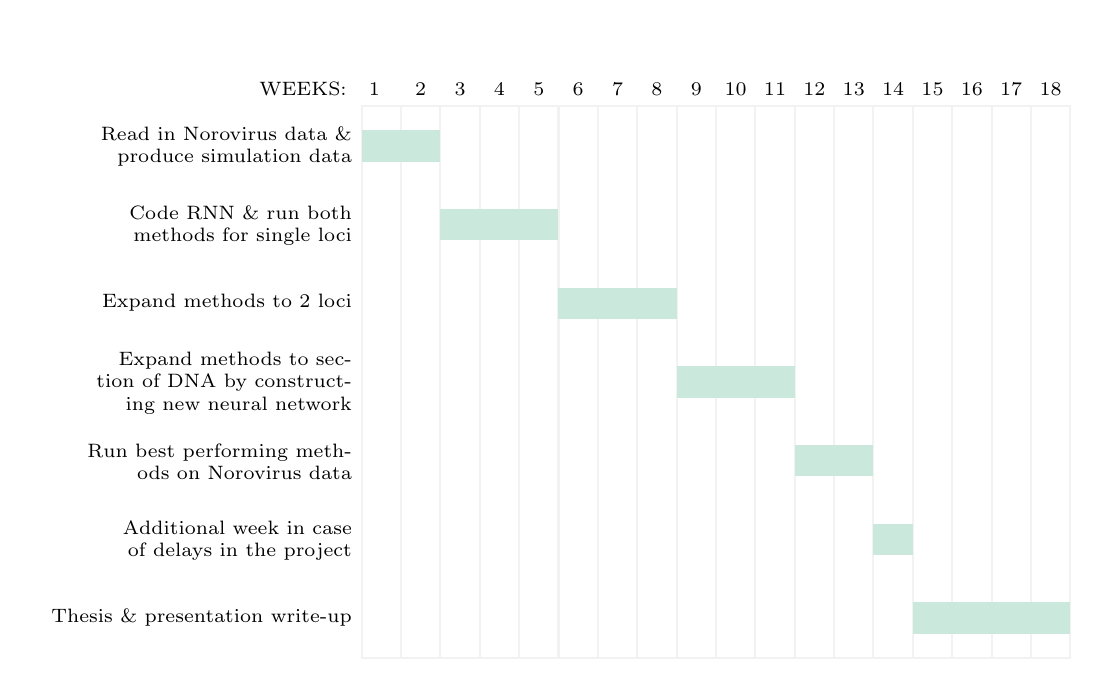
\begin{tikzpicture}
\begin{ganttchart}[canvas/.append style={fill=none, draw=black!5, line width=.75pt, alias=frame}, hgrid style/.style={draw=black!5, line width=.75pt}, vgrid={*1{draw=black!5, line width=.75pt}}, title/.style={draw=none, fill=none}, title/.style={draw=none, fill=none}, title label node/.append style={below=7pt}, include title in canvas=false, bar/.append style={draw=none, fill=duckegg}, title label font=\scriptsize, bar label node/.style={text width=4cm,align=right,font=\scriptsize\RaggedLeft,anchor=east},]{1}{18}
\gantttitle[title label node/.append style={below left=7pt and -3pt}]{WEEKS:\quad1}{1}
\gantttitlelist{2,...,18}{1}\\
\ganttbar{Read in Norovirus data \& produce simulation data}{1}{2}\\
\ganttbar{Code RNN \& run both methods for single loci}{3}{5}\\
\ganttbar{Expand methods to 2 loci}{6}{8}\\
\ganttbar{Expand methods to section of DNA by constructing new neural network}{9}{11}\\
\ganttbar{Run best performing methods on Norovirus data}{12}{13}\\
\ganttbar{Additional week in case of delays in the project}{14}{14}\\
\ganttbar{Thesis \& presentation write-up}{15}{18}
\end{ganttchart}
\end{tikzpicture}
\caption{Gantt chart for this project}
\end{figure}

\begin{onehalfspacing}
\linenumbers
\section{Itemised Budget}
\textbf{Research-related travel: £420}
\\
As I do not live at Silwood, and will be occupying desk space at Silwood instead of at the Crick Institute, where my main supervisor is mainly based, an outlay of £420, which accounts to 35 days return train fare (half the number of days that I expect to travel into Silwood over the course of 14 weeks) would be of great assistance to me.

\bibliographystyle{agsm}
\bibliography{Proposal_References}
\end{onehalfspacing}
\end{document}